\documentclass[twoside]{book}

% Packages required by doxygen
\usepackage{fixltx2e}
\usepackage{calc}
\usepackage{doxygen}
\usepackage[export]{adjustbox} % also loads graphicx
\usepackage{graphicx}
\usepackage[utf8]{inputenc}
\usepackage{makeidx}
\usepackage{multicol}
\usepackage{multirow}
\PassOptionsToPackage{warn}{textcomp}
\usepackage{textcomp}
\usepackage[nointegrals]{wasysym}
\usepackage[table]{xcolor}

% Font selection
\usepackage[T1]{fontenc}
\usepackage[scaled=.90]{helvet}
\usepackage{courier}
\usepackage{amssymb}
\usepackage{sectsty}
\renewcommand{\familydefault}{\sfdefault}
\allsectionsfont{%
  \fontseries{bc}\selectfont%
  \color{darkgray}%
}
\renewcommand{\DoxyLabelFont}{%
  \fontseries{bc}\selectfont%
  \color{darkgray}%
}
\newcommand{\+}{\discretionary{\mbox{\scriptsize$\hookleftarrow$}}{}{}}

% Page & text layout
\usepackage{geometry}
\geometry{%
  a4paper,%
  top=2.5cm,%
  bottom=2.5cm,%
  left=2.5cm,%
  right=2.5cm%
}
\tolerance=750
\hfuzz=15pt
\hbadness=750
\setlength{\emergencystretch}{15pt}
\setlength{\parindent}{0cm}
\setlength{\parskip}{3ex plus 2ex minus 2ex}
\makeatletter
\renewcommand{\paragraph}{%
  \@startsection{paragraph}{4}{0ex}{-1.0ex}{1.0ex}{%
    \normalfont\normalsize\bfseries\SS@parafont%
  }%
}
\renewcommand{\subparagraph}{%
  \@startsection{subparagraph}{5}{0ex}{-1.0ex}{1.0ex}{%
    \normalfont\normalsize\bfseries\SS@subparafont%
  }%
}
\makeatother

% Headers & footers
\usepackage{fancyhdr}
\pagestyle{fancyplain}
\fancyhead[LE]{\fancyplain{}{\bfseries\thepage}}
\fancyhead[CE]{\fancyplain{}{}}
\fancyhead[RE]{\fancyplain{}{\bfseries\leftmark}}
\fancyhead[LO]{\fancyplain{}{\bfseries\rightmark}}
\fancyhead[CO]{\fancyplain{}{}}
\fancyhead[RO]{\fancyplain{}{\bfseries\thepage}}
\fancyfoot[LE]{\fancyplain{}{}}
\fancyfoot[CE]{\fancyplain{}{}}
\fancyfoot[RE]{\fancyplain{}{\bfseries\scriptsize Generated by Doxygen }}
\fancyfoot[LO]{\fancyplain{}{\bfseries\scriptsize Generated by Doxygen }}
\fancyfoot[CO]{\fancyplain{}{}}
\fancyfoot[RO]{\fancyplain{}{}}
\renewcommand{\footrulewidth}{0.4pt}
\renewcommand{\chaptermark}[1]{%
  \markboth{#1}{}%
}
\renewcommand{\sectionmark}[1]{%
  \markright{\thesection\ #1}%
}

% Indices & bibliography
\usepackage{natbib}
\usepackage[titles]{tocloft}
\setcounter{tocdepth}{3}
\setcounter{secnumdepth}{5}
\makeindex

% Hyperlinks (required, but should be loaded last)
\usepackage{ifpdf}
\ifpdf
  \usepackage[pdftex,pagebackref=true]{hyperref}
\else
  \usepackage[ps2pdf,pagebackref=true]{hyperref}
\fi
\hypersetup{%
  colorlinks=true,%
  linkcolor=blue,%
  citecolor=blue,%
  unicode%
}

% Custom commands
\newcommand{\clearemptydoublepage}{%
  \newpage{\pagestyle{empty}\cleardoublepage}%
}

\usepackage{caption}
\captionsetup{labelsep=space,justification=centering,font={bf},singlelinecheck=off,skip=4pt,position=top}

%===== C O N T E N T S =====

\begin{document}

% Titlepage & ToC
\hypersetup{pageanchor=false,
             bookmarksnumbered=true,
             pdfencoding=unicode
            }
\pagenumbering{alph}
\begin{titlepage}
\vspace*{7cm}
\begin{center}%
{\Large Konenako }\\
\vspace*{1cm}
{\large Generated by Doxygen 1.8.13}\\
\end{center}
\end{titlepage}
\clearemptydoublepage
\pagenumbering{roman}
\tableofcontents
\clearemptydoublepage
\pagenumbering{arabic}
\hypersetup{pageanchor=true}

%--- Begin generated contents ---
\chapter{Documentation Tips}
\label{index}\hypertarget{index}{}\subsection*{How to document the project}

This is a brief instruction for making doxygen documents.

\subsubsection*{Tags}

You can use tags in Python files, and Doxygen will list them under \href{pages.html}{\tt Related Pages}. \begin{DoxyVerb}## @'bug Lets fix this  
\end{DoxyVerb}


Some useful tags\+:
\begin{DoxyItemize}
\item \begin{DoxyRefDesc}{Bug}
\item[\hyperlink{bug__bug000001}{Bug}]\end{DoxyRefDesc}
\begin{DoxyRefDesc}{Todo}
\item[\hyperlink{todo__todo000001}{Todo}]\end{DoxyRefDesc}
\begin{DoxyRefDesc}{Test}
\item[\hyperlink{test__test000001}{Test}]\end{DoxyRefDesc}

\end{DoxyItemize}

You can run doxygen in root with \begin{DoxyVerb}doxygen    
\end{DoxyVerb}


The documentation files can be found in the documentation-\/folder.

\href{https://github.com/Konenako/Ohtuprojekti-kesa2020}{\tt Project in github} 
\chapter{Usage}
\label{md_rostest_README}
\Hypertarget{md_rostest_README}
Setup R\+OS catkin workspace, {\ttfamily git clone} to {\ttfamily catkin\+\_\+ws/src/} and build the catkin workspace.

{\ttfamily poetry shell} 
\begin{DoxyCode}
source ../../devel/setup.bash
cd rostest
rosrun rostest main.py
\end{DoxyCode}


\subsection*{Docker}

Building the image

{\ttfamily sudo docker build -\/-\/tag rostest\+:1.\+0 .}

Create network for communicating with roscore

{\ttfamily sudo docker network create rosnet}

Start up roscore 
\begin{DoxyCode}
sudo docker run -it --rm \(\backslash\)
--net rosnet \(\backslash\)
--name master \(\backslash\)
ros:melodic-ros-core \(\backslash\)
roscore
\end{DoxyCode}
 Start up rostest node in another console 
\begin{DoxyCode}
sudo docker run -it --rm \(\backslash\)
    --net rosnet \(\backslash\)
    --name rostest \(\backslash\)
    --env ROS\_HOSTNAME=rostest \(\backslash\)
    --env ROS\_MASTER\_URI=http://master:11311 \(\backslash\)
    rostest:1.0
\end{DoxyCode}
 Attaching camera devices to the container can be done by adding parameters to node container startup

{\ttfamily -\/-\/device} argument, for example {\ttfamily -\/-\/device /dev/video0}

\subsubsection*{Docker compose}

Alternatively the above can be done with docker compose, with the following on the root directory of the project.

{\ttfamily docker-\/compose build}

{\ttfamily docker-\/compose up}

For sending messages to rostest.\+py attach to input container with another terminal\+:

{\ttfamily sudo docker attach rosinput}

For seeing recieved messages in separate terminal use\+:

{\ttfamily sudo docker attach rostest}

For seeing recieved information about the objects use\+:

{\ttfamily sudo docker attach rosprinter}

Attaching devices like webcams \href{https://docs.docker.com/compose/compose-file/#devices}{\tt https\+://docs.\+docker.\+com/compose/compose-\/file/\#devices}

\subsection*{Versions}

Tested to work on Docker version 19.\+03.\+8-\/ce and Docker-\/compose version 1.\+25.\+5 
\chapter{Test List}
\label{test}
\Hypertarget{test}

\begin{DoxyRefList}
\item[\label{test__test000001}%
\Hypertarget{test__test000001}%
page \hyperlink{index}{Documentation Tips} ]
\end{DoxyRefList}
\chapter{Todo List}
\label{todo}
\Hypertarget{todo}

\begin{DoxyRefList}
\item[\label{todo__todo000001}%
\Hypertarget{todo__todo000001}%
page \hyperlink{index}{Documentation Tips} ]
\begin{DoxyItemize}
\item 
\end{DoxyItemize}
\end{DoxyRefList}
\chapter{Bug List}
\label{bug}
\Hypertarget{bug}

\begin{DoxyRefList}
\item[\label{bug__bug000001}%
\Hypertarget{bug__bug000001}%
page \hyperlink{index}{Documentation Tips} ]
\begin{DoxyItemize}
\item 
\end{DoxyItemize}
\end{DoxyRefList}
\chapter{Namespace Index}
\section{Namespace List}
Here is a list of all namespaces with brief descriptions\+:\begin{DoxyCompactList}
\item\contentsline{section}{\hyperlink{namespacecamera}{camera} }{\pageref{namespacecamera}}{}
\item\contentsline{section}{\hyperlink{namespaceimage__converter}{image\+\_\+converter} }{\pageref{namespaceimage__converter}}{}
\item\contentsline{section}{\hyperlink{namespaceinput}{input} }{\pageref{namespaceinput}}{}
\item\contentsline{section}{\hyperlink{namespacemain}{main} }{\pageref{namespacemain}}{}
\item\contentsline{section}{\hyperlink{namespaceobject__detection}{object\+\_\+detection} }{\pageref{namespaceobject__detection}}{}
\item\contentsline{section}{\hyperlink{namespaceobject__detector}{object\+\_\+detector} }{\pageref{namespaceobject__detector}}{}
\item\contentsline{section}{\hyperlink{namespaceprinter}{printer} }{\pageref{namespaceprinter}}{}
\item\contentsline{section}{\hyperlink{namespaceqr}{qr} }{\pageref{namespaceqr}}{}
\item\contentsline{section}{\hyperlink{namespaceqr__detector}{qr\+\_\+detector} }{\pageref{namespaceqr__detector}}{}
\item\contentsline{section}{\hyperlink{namespaceqr__node}{qr\+\_\+node} }{\pageref{namespaceqr__node}}{}
\item\contentsline{section}{\hyperlink{namespacetests}{tests} }{\pageref{namespacetests}}{}
\item\contentsline{section}{\hyperlink{namespacetests_1_1test__object__detector}{tests.\+test\+\_\+object\+\_\+detector} }{\pageref{namespacetests_1_1test__object__detector}}{}
\item\contentsline{section}{\hyperlink{namespacetests_1_1test__qr__detector}{tests.\+test\+\_\+qr\+\_\+detector} }{\pageref{namespacetests_1_1test__qr__detector}}{}
\end{DoxyCompactList}

\chapter{Hierarchical Index}
\section{Class Hierarchy}
This inheritance list is sorted roughly, but not completely, alphabetically\+:\begin{DoxyCompactList}
\item \contentsline{section}{object\+\_\+detector.\+Object\+Detector}{\pageref{classobject__detector_1_1ObjectDetector}}{}
\item \contentsline{section}{qr\+\_\+node.\+Q\+R\+Reader}{\pageref{classqr__node_1_1QRReader}}{}
\item Test\+Case\begin{DoxyCompactList}
\item \contentsline{section}{tests.\+test\+\_\+object\+\_\+detector.\+Detector}{\pageref{classtests_1_1test__object__detector_1_1Detector}}{}
\item \contentsline{section}{tests.\+test\+\_\+qr\+\_\+detector.\+Q\+R\+Code\+Detector}{\pageref{classtests_1_1test__qr__detector_1_1QRCodeDetector}}{}
\end{DoxyCompactList}
\end{DoxyCompactList}

\chapter{Class Index}
\section{Class List}
Here are the classes, structs, unions and interfaces with brief descriptions\+:\begin{DoxyCompactList}
\item\contentsline{section}{\hyperlink{classtests_1_1test__object__detector_1_1Detector}{tests.\+test\+\_\+object\+\_\+detector.\+Detector} }{\pageref{classtests_1_1test__object__detector_1_1Detector}}{}
\item\contentsline{section}{\hyperlink{classobject__detector_1_1ObjectDetector}{object\+\_\+detector.\+Object\+Detector} }{\pageref{classobject__detector_1_1ObjectDetector}}{}
\item\contentsline{section}{\hyperlink{classtests_1_1test__qr__detector_1_1QRCodeDetector}{tests.\+test\+\_\+qr\+\_\+detector.\+Q\+R\+Code\+Detector} }{\pageref{classtests_1_1test__qr__detector_1_1QRCodeDetector}}{}
\item\contentsline{section}{\hyperlink{classqr__node_1_1QRReader}{qr\+\_\+node.\+Q\+R\+Reader} }{\pageref{classqr__node_1_1QRReader}}{}
\end{DoxyCompactList}

\chapter{File Index}
\section{File List}
Here is a list of all files with brief descriptions\+:\begin{DoxyCompactList}
\item\contentsline{section}{rostest/scripts/\hyperlink{input_8py}{input.\+py} }{\pageref{input_8py}}{}
\item\contentsline{section}{rostest/scripts/\hyperlink{main_8py}{main.\+py} }{\pageref{main_8py}}{}
\item\contentsline{section}{rostest/scripts/\hyperlink{object__detector_8py}{object\+\_\+detector.\+py} }{\pageref{object__detector_8py}}{}
\item\contentsline{section}{rostest/scripts/\hyperlink{printer_8py}{printer.\+py} }{\pageref{printer_8py}}{}
\item\contentsline{section}{rostest/tests/\hyperlink{____init_____8py}{\+\_\+\+\_\+init\+\_\+\+\_\+.\+py} }{\pageref{____init_____8py}}{}
\item\contentsline{section}{rostest/tests/\hyperlink{test__object__detector_8py}{test\+\_\+object\+\_\+detector.\+py} }{\pageref{test__object__detector_8py}}{}
\end{DoxyCompactList}

\chapter{Namespace Documentation}
\hypertarget{namespaceinput}{}\section{input Namespace Reference}
\label{namespaceinput}\index{input@{input}}
\subsection*{Functions}
\begin{DoxyCompactItemize}
\item 
def \hyperlink{namespaceinput_a93769ba24482b0fb5fb527f7e6b9e98f}{send\+\_\+message} ()
\item 
def \hyperlink{namespaceinput_a0e027bacb0e23962a92058b4de7df02d}{send\+\_\+frequency} ()
\item 
def \hyperlink{namespaceinput_a03ee62d50c865b3932ded679640747c9}{send\+\_\+qr\+\_\+frequency} ()
\item 
def \hyperlink{namespaceinput_acf8fe4c0bb6a777022f311c22f311770}{run} ()
\item 
def \hyperlink{namespaceinput_aea99d1687a0fd65c426df890f7c4e294}{init} ()
\end{DoxyCompactItemize}
\subsection*{Variables}
\begin{DoxyCompactItemize}
\item 
\hyperlink{namespaceinput_a9d4e412eda6375c7b27aeeccba8a2839}{message\+\_\+receiver} = None
\item 
\hyperlink{namespaceinput_ab769f6cd43885395710f5a098d8e890b}{frequency\+\_\+changer} = None
\item 
\hyperlink{namespaceinput_ac8b28af0ed72d501832d19897067fb3c}{qr\+\_\+frequency\+\_\+changer} = None
\end{DoxyCompactItemize}


\subsection{Function Documentation}
\mbox{\Hypertarget{namespaceinput_aea99d1687a0fd65c426df890f7c4e294}\label{namespaceinput_aea99d1687a0fd65c426df890f7c4e294}} 
\index{input@{input}!init@{init}}
\index{init@{init}!input@{input}}
\subsubsection{\texorpdfstring{init()}{init()}}
{\footnotesize\ttfamily def input.\+init (\begin{DoxyParamCaption}{ }\end{DoxyParamCaption})}

\mbox{\Hypertarget{namespaceinput_acf8fe4c0bb6a777022f311c22f311770}\label{namespaceinput_acf8fe4c0bb6a777022f311c22f311770}} 
\index{input@{input}!run@{run}}
\index{run@{run}!input@{input}}
\subsubsection{\texorpdfstring{run()}{run()}}
{\footnotesize\ttfamily def input.\+run (\begin{DoxyParamCaption}{ }\end{DoxyParamCaption})}

\mbox{\Hypertarget{namespaceinput_a0e027bacb0e23962a92058b4de7df02d}\label{namespaceinput_a0e027bacb0e23962a92058b4de7df02d}} 
\index{input@{input}!send\+\_\+frequency@{send\+\_\+frequency}}
\index{send\+\_\+frequency@{send\+\_\+frequency}!input@{input}}
\subsubsection{\texorpdfstring{send\+\_\+frequency()}{send\_frequency()}}
{\footnotesize\ttfamily def input.\+send\+\_\+frequency (\begin{DoxyParamCaption}{ }\end{DoxyParamCaption})}

\mbox{\Hypertarget{namespaceinput_a93769ba24482b0fb5fb527f7e6b9e98f}\label{namespaceinput_a93769ba24482b0fb5fb527f7e6b9e98f}} 
\index{input@{input}!send\+\_\+message@{send\+\_\+message}}
\index{send\+\_\+message@{send\+\_\+message}!input@{input}}
\subsubsection{\texorpdfstring{send\+\_\+message()}{send\_message()}}
{\footnotesize\ttfamily def input.\+send\+\_\+message (\begin{DoxyParamCaption}{ }\end{DoxyParamCaption})}

\mbox{\Hypertarget{namespaceinput_a03ee62d50c865b3932ded679640747c9}\label{namespaceinput_a03ee62d50c865b3932ded679640747c9}} 
\index{input@{input}!send\+\_\+qr\+\_\+frequency@{send\+\_\+qr\+\_\+frequency}}
\index{send\+\_\+qr\+\_\+frequency@{send\+\_\+qr\+\_\+frequency}!input@{input}}
\subsubsection{\texorpdfstring{send\+\_\+qr\+\_\+frequency()}{send\_qr\_frequency()}}
{\footnotesize\ttfamily def input.\+send\+\_\+qr\+\_\+frequency (\begin{DoxyParamCaption}{ }\end{DoxyParamCaption})}



\subsection{Variable Documentation}
\mbox{\Hypertarget{namespaceinput_ab769f6cd43885395710f5a098d8e890b}\label{namespaceinput_ab769f6cd43885395710f5a098d8e890b}} 
\index{input@{input}!frequency\+\_\+changer@{frequency\+\_\+changer}}
\index{frequency\+\_\+changer@{frequency\+\_\+changer}!input@{input}}
\subsubsection{\texorpdfstring{frequency\+\_\+changer}{frequency\_changer}}
{\footnotesize\ttfamily input.\+frequency\+\_\+changer = None}

\mbox{\Hypertarget{namespaceinput_a9d4e412eda6375c7b27aeeccba8a2839}\label{namespaceinput_a9d4e412eda6375c7b27aeeccba8a2839}} 
\index{input@{input}!message\+\_\+receiver@{message\+\_\+receiver}}
\index{message\+\_\+receiver@{message\+\_\+receiver}!input@{input}}
\subsubsection{\texorpdfstring{message\+\_\+receiver}{message\_receiver}}
{\footnotesize\ttfamily input.\+message\+\_\+receiver = None}

\mbox{\Hypertarget{namespaceinput_ac8b28af0ed72d501832d19897067fb3c}\label{namespaceinput_ac8b28af0ed72d501832d19897067fb3c}} 
\index{input@{input}!qr\+\_\+frequency\+\_\+changer@{qr\+\_\+frequency\+\_\+changer}}
\index{qr\+\_\+frequency\+\_\+changer@{qr\+\_\+frequency\+\_\+changer}!input@{input}}
\subsubsection{\texorpdfstring{qr\+\_\+frequency\+\_\+changer}{qr\_frequency\_changer}}
{\footnotesize\ttfamily input.\+qr\+\_\+frequency\+\_\+changer = None}


\hypertarget{namespacemain}{}\section{main Namespace Reference}
\label{namespacemain}\index{main@{main}}
\subsection*{Functions}
\begin{DoxyCompactItemize}
\item 
def \hyperlink{namespacemain_a0fe3fdb168f80f23bd787b6a6645d063}{print\+\_\+input} (input)
\item 
def \hyperlink{namespacemain_a191dcce5a995145c51a8935645d7de97}{change\+\_\+frequency} (new\+\_\+frequency)
\item 
def \hyperlink{namespacemain_a1fa92828a6a055fa38390012ffdd2b87}{run}
\end{DoxyCompactItemize}
\subsection*{Variables}
\begin{DoxyCompactItemize}
\item 
int \hyperlink{namespacemain_a57172d55d7c1b86fc48bcbc6c3783efb}{run\+\_\+frequency} = 1
\item 
float \hyperlink{namespacemain_a9ec7279618de6ff9195552f460584339}{period} = 1.\+0 / \hyperlink{namespacemain_a57172d55d7c1b86fc48bcbc6c3783efb}{run\+\_\+frequency}
\item 
string \hyperlink{namespacemain_a75667a1170a74674aa6f7fa04dca3f51}{source} = \char`\"{}test.\+mp4\char`\"{}
\end{DoxyCompactItemize}


\subsection{Function Documentation}
\mbox{\Hypertarget{namespacemain_a191dcce5a995145c51a8935645d7de97}\label{namespacemain_a191dcce5a995145c51a8935645d7de97}} 
\index{main@{main}!change\+\_\+frequency@{change\+\_\+frequency}}
\index{change\+\_\+frequency@{change\+\_\+frequency}!main@{main}}
\subsubsection{\texorpdfstring{change\+\_\+frequency()}{change\_frequency()}}
{\footnotesize\ttfamily def main.\+change\+\_\+frequency (\begin{DoxyParamCaption}\item[{}]{new\+\_\+frequency }\end{DoxyParamCaption})}

\mbox{\Hypertarget{namespacemain_a0fe3fdb168f80f23bd787b6a6645d063}\label{namespacemain_a0fe3fdb168f80f23bd787b6a6645d063}} 
\index{main@{main}!print\+\_\+input@{print\+\_\+input}}
\index{print\+\_\+input@{print\+\_\+input}!main@{main}}
\subsubsection{\texorpdfstring{print\+\_\+input()}{print\_input()}}
{\footnotesize\ttfamily def main.\+print\+\_\+input (\begin{DoxyParamCaption}\item[{}]{input }\end{DoxyParamCaption})}

\mbox{\Hypertarget{namespacemain_a1fa92828a6a055fa38390012ffdd2b87}\label{namespacemain_a1fa92828a6a055fa38390012ffdd2b87}} 
\index{main@{main}!run@{run}}
\index{run@{run}!main@{main}}
\subsubsection{\texorpdfstring{run()}{run()}}
{\footnotesize\ttfamily def main.\+run (\begin{DoxyParamCaption}\item[{}]{showgui }\end{DoxyParamCaption})}



\subsection{Variable Documentation}
\mbox{\Hypertarget{namespacemain_a9ec7279618de6ff9195552f460584339}\label{namespacemain_a9ec7279618de6ff9195552f460584339}} 
\index{main@{main}!period@{period}}
\index{period@{period}!main@{main}}
\subsubsection{\texorpdfstring{period}{period}}
{\footnotesize\ttfamily float main.\+period = 1.\+0 / \hyperlink{namespacemain_a57172d55d7c1b86fc48bcbc6c3783efb}{run\+\_\+frequency}}

\mbox{\Hypertarget{namespacemain_a57172d55d7c1b86fc48bcbc6c3783efb}\label{namespacemain_a57172d55d7c1b86fc48bcbc6c3783efb}} 
\index{main@{main}!run\+\_\+frequency@{run\+\_\+frequency}}
\index{run\+\_\+frequency@{run\+\_\+frequency}!main@{main}}
\subsubsection{\texorpdfstring{run\+\_\+frequency}{run\_frequency}}
{\footnotesize\ttfamily int main.\+run\+\_\+frequency = 1}

\mbox{\Hypertarget{namespacemain_a75667a1170a74674aa6f7fa04dca3f51}\label{namespacemain_a75667a1170a74674aa6f7fa04dca3f51}} 
\index{main@{main}!source@{source}}
\index{source@{source}!main@{main}}
\subsubsection{\texorpdfstring{source}{source}}
{\footnotesize\ttfamily string main.\+source = \char`\"{}test.\+mp4\char`\"{}}


\hypertarget{namespaceobject__detector}{}\section{object\+\_\+detector Namespace Reference}
\label{namespaceobject__detector}\index{object\+\_\+detector@{object\+\_\+detector}}
\subsection*{Classes}
\begin{DoxyCompactItemize}
\item 
class \hyperlink{classobject__detector_1_1ObjectDetector}{Object\+Detector}
\end{DoxyCompactItemize}

\hypertarget{namespaceprinter}{}\section{printer Namespace Reference}
\label{namespaceprinter}\index{printer@{printer}}
\subsection*{Functions}
\begin{DoxyCompactItemize}
\item 
def \hyperlink{namespaceprinter_a3eb27980abedac28745fb43f61bfe198}{printer} (obs)
\item 
def \hyperlink{namespaceprinter_abd8f2589552090a9b3b5f2cd1f941b8b}{run} ()
\end{DoxyCompactItemize}


\subsection{Function Documentation}
\mbox{\Hypertarget{namespaceprinter_a3eb27980abedac28745fb43f61bfe198}\label{namespaceprinter_a3eb27980abedac28745fb43f61bfe198}} 
\index{printer@{printer}!printer@{printer}}
\index{printer@{printer}!printer@{printer}}
\subsubsection{\texorpdfstring{printer()}{printer()}}
{\footnotesize\ttfamily def printer.\+printer (\begin{DoxyParamCaption}\item[{}]{obs }\end{DoxyParamCaption})}

\mbox{\Hypertarget{namespaceprinter_abd8f2589552090a9b3b5f2cd1f941b8b}\label{namespaceprinter_abd8f2589552090a9b3b5f2cd1f941b8b}} 
\index{printer@{printer}!run@{run}}
\index{run@{run}!printer@{printer}}
\subsubsection{\texorpdfstring{run()}{run()}}
{\footnotesize\ttfamily def printer.\+run (\begin{DoxyParamCaption}{ }\end{DoxyParamCaption})}


\hypertarget{namespacetests}{}\section{tests Namespace Reference}
\label{namespacetests}\index{tests@{tests}}
\subsection*{Namespaces}
\begin{DoxyCompactItemize}
\item 
 \hyperlink{namespacetests_1_1test__object__detector}{test\+\_\+object\+\_\+detector}
\end{DoxyCompactItemize}

\hypertarget{namespacetests_1_1test__object__detector}{}\section{tests.\+test\+\_\+object\+\_\+detector Namespace Reference}
\label{namespacetests_1_1test__object__detector}\index{tests.\+test\+\_\+object\+\_\+detector@{tests.\+test\+\_\+object\+\_\+detector}}
\subsection*{Classes}
\begin{DoxyCompactItemize}
\item 
class \hyperlink{classtests_1_1test__object__detector_1_1Detector}{Detector}
\end{DoxyCompactItemize}

\chapter{Class Documentation}
\hypertarget{classtests_1_1test__object__detector_1_1Detector}{}\section{tests.\+test\+\_\+object\+\_\+detector.\+Detector Class Reference}
\label{classtests_1_1test__object__detector_1_1Detector}\index{tests.\+test\+\_\+object\+\_\+detector.\+Detector@{tests.\+test\+\_\+object\+\_\+detector.\+Detector}}


Inheritance diagram for tests.\+test\+\_\+object\+\_\+detector.\+Detector\+:
\nopagebreak
\begin{figure}[H]
\begin{center}
\leavevmode
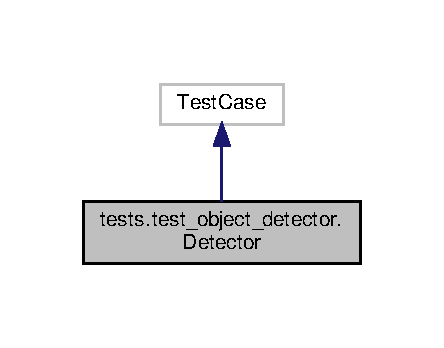
\includegraphics[width=213pt]{classtests_1_1test__object__detector_1_1Detector__inherit__graph}
\end{center}
\end{figure}


Collaboration diagram for tests.\+test\+\_\+object\+\_\+detector.\+Detector\+:
\nopagebreak
\begin{figure}[H]
\begin{center}
\leavevmode
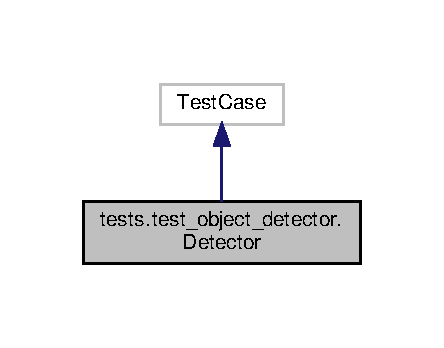
\includegraphics[width=213pt]{classtests_1_1test__object__detector_1_1Detector__coll__graph}
\end{center}
\end{figure}
\subsection*{Public Member Functions}
\begin{DoxyCompactItemize}
\item 
def \hyperlink{classtests_1_1test__object__detector_1_1Detector_afa15ba2941421016d69736377f867233}{test\+\_\+detect\+\_\+cow\+\_\+banana} (self)
\end{DoxyCompactItemize}


\subsection{Member Function Documentation}
\mbox{\Hypertarget{classtests_1_1test__object__detector_1_1Detector_afa15ba2941421016d69736377f867233}\label{classtests_1_1test__object__detector_1_1Detector_afa15ba2941421016d69736377f867233}} 
\index{tests\+::test\+\_\+object\+\_\+detector\+::\+Detector@{tests\+::test\+\_\+object\+\_\+detector\+::\+Detector}!test\+\_\+detect\+\_\+cow\+\_\+banana@{test\+\_\+detect\+\_\+cow\+\_\+banana}}
\index{test\+\_\+detect\+\_\+cow\+\_\+banana@{test\+\_\+detect\+\_\+cow\+\_\+banana}!tests\+::test\+\_\+object\+\_\+detector\+::\+Detector@{tests\+::test\+\_\+object\+\_\+detector\+::\+Detector}}
\subsubsection{\texorpdfstring{test\+\_\+detect\+\_\+cow\+\_\+banana()}{test\_detect\_cow\_banana()}}
{\footnotesize\ttfamily def tests.\+test\+\_\+object\+\_\+detector.\+Detector.\+test\+\_\+detect\+\_\+cow\+\_\+banana (\begin{DoxyParamCaption}\item[{}]{self }\end{DoxyParamCaption})}



The documentation for this class was generated from the following file\+:\begin{DoxyCompactItemize}
\item 
rostest/tests/\hyperlink{test__object__detector_8py}{test\+\_\+object\+\_\+detector.\+py}\end{DoxyCompactItemize}

\hypertarget{classobject__detector_1_1ObjectDetector}{}\section{object\+\_\+detector.\+Object\+Detector Class Reference}
\label{classobject__detector_1_1ObjectDetector}\index{object\+\_\+detector.\+Object\+Detector@{object\+\_\+detector.\+Object\+Detector}}
\subsection*{Public Member Functions}
\begin{DoxyCompactItemize}
\item 
def \hyperlink{classobject__detector_1_1ObjectDetector_a798b45f16d50dc89ba57bfa4369fd01d}{\+\_\+\+\_\+init\+\_\+\+\_\+}
\item 
def \hyperlink{classobject__detector_1_1ObjectDetector_aaad9724f89d4803c10c0ab346c6b9121}{load\+\_\+labels}
\item 
def \hyperlink{classobject__detector_1_1ObjectDetector_a230551f06d7906793bfa1e44654fdefe}{load\+\_\+model}
\item 
def \hyperlink{classobject__detector_1_1ObjectDetector_ab03e2a22955f2438ee905377938a72ee}{detect} (self, img)
\end{DoxyCompactItemize}
\subsection*{Public Attributes}
\begin{DoxyCompactItemize}
\item 
\hyperlink{classobject__detector_1_1ObjectDetector_ae111e0c0f55d86a47ed7209ca249f5a2}{labels}
\item 
\hyperlink{classobject__detector_1_1ObjectDetector_a64136107df666740de86c933278a8460}{interpreter}
\item 
\hyperlink{classobject__detector_1_1ObjectDetector_abffe93fe0cff55ce4038679483cab0a2}{input\+\_\+details}
\item 
\hyperlink{classobject__detector_1_1ObjectDetector_a167991814c90ee1c872fad8ac9a0b6ec}{output\+\_\+details}
\end{DoxyCompactItemize}


\subsection{Constructor \& Destructor Documentation}
\mbox{\Hypertarget{classobject__detector_1_1ObjectDetector_a798b45f16d50dc89ba57bfa4369fd01d}\label{classobject__detector_1_1ObjectDetector_a798b45f16d50dc89ba57bfa4369fd01d}} 
\index{object\+\_\+detector\+::\+Object\+Detector@{object\+\_\+detector\+::\+Object\+Detector}!\+\_\+\+\_\+init\+\_\+\+\_\+@{\+\_\+\+\_\+init\+\_\+\+\_\+}}
\index{\+\_\+\+\_\+init\+\_\+\+\_\+@{\+\_\+\+\_\+init\+\_\+\+\_\+}!object\+\_\+detector\+::\+Object\+Detector@{object\+\_\+detector\+::\+Object\+Detector}}
\subsubsection{\texorpdfstring{\+\_\+\+\_\+init\+\_\+\+\_\+()}{\_\_init\_\_()}}
{\footnotesize\ttfamily def object\+\_\+detector.\+Object\+Detector.\+\_\+\+\_\+init\+\_\+\+\_\+ (\begin{DoxyParamCaption}\item[{}]{self,  }\item[{}]{model\+\_\+path }\end{DoxyParamCaption})}



\subsection{Member Function Documentation}
\mbox{\Hypertarget{classobject__detector_1_1ObjectDetector_ab03e2a22955f2438ee905377938a72ee}\label{classobject__detector_1_1ObjectDetector_ab03e2a22955f2438ee905377938a72ee}} 
\index{object\+\_\+detector\+::\+Object\+Detector@{object\+\_\+detector\+::\+Object\+Detector}!detect@{detect}}
\index{detect@{detect}!object\+\_\+detector\+::\+Object\+Detector@{object\+\_\+detector\+::\+Object\+Detector}}
\subsubsection{\texorpdfstring{detect()}{detect()}}
{\footnotesize\ttfamily def object\+\_\+detector.\+Object\+Detector.\+detect (\begin{DoxyParamCaption}\item[{}]{self,  }\item[{}]{img }\end{DoxyParamCaption})}

\mbox{\Hypertarget{classobject__detector_1_1ObjectDetector_aaad9724f89d4803c10c0ab346c6b9121}\label{classobject__detector_1_1ObjectDetector_aaad9724f89d4803c10c0ab346c6b9121}} 
\index{object\+\_\+detector\+::\+Object\+Detector@{object\+\_\+detector\+::\+Object\+Detector}!load\+\_\+labels@{load\+\_\+labels}}
\index{load\+\_\+labels@{load\+\_\+labels}!object\+\_\+detector\+::\+Object\+Detector@{object\+\_\+detector\+::\+Object\+Detector}}
\subsubsection{\texorpdfstring{load\+\_\+labels()}{load\_labels()}}
{\footnotesize\ttfamily def object\+\_\+detector.\+Object\+Detector.\+load\+\_\+labels (\begin{DoxyParamCaption}\item[{}]{self,  }\item[{}]{label\+\_\+path }\end{DoxyParamCaption})}

\mbox{\Hypertarget{classobject__detector_1_1ObjectDetector_a230551f06d7906793bfa1e44654fdefe}\label{classobject__detector_1_1ObjectDetector_a230551f06d7906793bfa1e44654fdefe}} 
\index{object\+\_\+detector\+::\+Object\+Detector@{object\+\_\+detector\+::\+Object\+Detector}!load\+\_\+model@{load\+\_\+model}}
\index{load\+\_\+model@{load\+\_\+model}!object\+\_\+detector\+::\+Object\+Detector@{object\+\_\+detector\+::\+Object\+Detector}}
\subsubsection{\texorpdfstring{load\+\_\+model()}{load\_model()}}
{\footnotesize\ttfamily def object\+\_\+detector.\+Object\+Detector.\+load\+\_\+model (\begin{DoxyParamCaption}\item[{}]{self,  }\item[{}]{model\+\_\+path }\end{DoxyParamCaption})}



\subsection{Member Data Documentation}
\mbox{\Hypertarget{classobject__detector_1_1ObjectDetector_abffe93fe0cff55ce4038679483cab0a2}\label{classobject__detector_1_1ObjectDetector_abffe93fe0cff55ce4038679483cab0a2}} 
\index{object\+\_\+detector\+::\+Object\+Detector@{object\+\_\+detector\+::\+Object\+Detector}!input\+\_\+details@{input\+\_\+details}}
\index{input\+\_\+details@{input\+\_\+details}!object\+\_\+detector\+::\+Object\+Detector@{object\+\_\+detector\+::\+Object\+Detector}}
\subsubsection{\texorpdfstring{input\+\_\+details}{input\_details}}
{\footnotesize\ttfamily object\+\_\+detector.\+Object\+Detector.\+input\+\_\+details}

\mbox{\Hypertarget{classobject__detector_1_1ObjectDetector_a64136107df666740de86c933278a8460}\label{classobject__detector_1_1ObjectDetector_a64136107df666740de86c933278a8460}} 
\index{object\+\_\+detector\+::\+Object\+Detector@{object\+\_\+detector\+::\+Object\+Detector}!interpreter@{interpreter}}
\index{interpreter@{interpreter}!object\+\_\+detector\+::\+Object\+Detector@{object\+\_\+detector\+::\+Object\+Detector}}
\subsubsection{\texorpdfstring{interpreter}{interpreter}}
{\footnotesize\ttfamily object\+\_\+detector.\+Object\+Detector.\+interpreter}

\mbox{\Hypertarget{classobject__detector_1_1ObjectDetector_ae111e0c0f55d86a47ed7209ca249f5a2}\label{classobject__detector_1_1ObjectDetector_ae111e0c0f55d86a47ed7209ca249f5a2}} 
\index{object\+\_\+detector\+::\+Object\+Detector@{object\+\_\+detector\+::\+Object\+Detector}!labels@{labels}}
\index{labels@{labels}!object\+\_\+detector\+::\+Object\+Detector@{object\+\_\+detector\+::\+Object\+Detector}}
\subsubsection{\texorpdfstring{labels}{labels}}
{\footnotesize\ttfamily object\+\_\+detector.\+Object\+Detector.\+labels}

\mbox{\Hypertarget{classobject__detector_1_1ObjectDetector_a167991814c90ee1c872fad8ac9a0b6ec}\label{classobject__detector_1_1ObjectDetector_a167991814c90ee1c872fad8ac9a0b6ec}} 
\index{object\+\_\+detector\+::\+Object\+Detector@{object\+\_\+detector\+::\+Object\+Detector}!output\+\_\+details@{output\+\_\+details}}
\index{output\+\_\+details@{output\+\_\+details}!object\+\_\+detector\+::\+Object\+Detector@{object\+\_\+detector\+::\+Object\+Detector}}
\subsubsection{\texorpdfstring{output\+\_\+details}{output\_details}}
{\footnotesize\ttfamily object\+\_\+detector.\+Object\+Detector.\+output\+\_\+details}



The documentation for this class was generated from the following file\+:\begin{DoxyCompactItemize}
\item 
rostest/scripts/\hyperlink{object__detector_8py}{object\+\_\+detector.\+py}\end{DoxyCompactItemize}

\chapter{File Documentation}
\hypertarget{mainpage_8md}{}\section{rostest/mainpage.md File Reference}
\label{mainpage_8md}\index{rostest/mainpage.\+md@{rostest/mainpage.\+md}}

\hypertarget{README_8md}{}\section{rostest/\+R\+E\+A\+D\+ME.md File Reference}
\label{README_8md}\index{rostest/\+R\+E\+A\+D\+M\+E.\+md@{rostest/\+R\+E\+A\+D\+M\+E.\+md}}

\hypertarget{input_8py}{}\section{rostest/scripts/input.py File Reference}
\label{input_8py}\index{rostest/scripts/input.\+py@{rostest/scripts/input.\+py}}
\subsection*{Namespaces}
\begin{DoxyCompactItemize}
\item 
 \hyperlink{namespaceinput}{input}
\end{DoxyCompactItemize}
\subsection*{Functions}
\begin{DoxyCompactItemize}
\item 
def \hyperlink{namespaceinput_a93769ba24482b0fb5fb527f7e6b9e98f}{input.\+send\+\_\+message} ()
\item 
def \hyperlink{namespaceinput_a0e027bacb0e23962a92058b4de7df02d}{input.\+send\+\_\+frequency} ()
\item 
def \hyperlink{namespaceinput_a03ee62d50c865b3932ded679640747c9}{input.\+send\+\_\+qr\+\_\+frequency} ()
\item 
def \hyperlink{namespaceinput_acf8fe4c0bb6a777022f311c22f311770}{input.\+run} ()
\item 
def \hyperlink{namespaceinput_aea99d1687a0fd65c426df890f7c4e294}{input.\+init} ()
\end{DoxyCompactItemize}
\subsection*{Variables}
\begin{DoxyCompactItemize}
\item 
\hyperlink{namespaceinput_a9d4e412eda6375c7b27aeeccba8a2839}{input.\+message\+\_\+receiver} = None
\item 
\hyperlink{namespaceinput_ab769f6cd43885395710f5a098d8e890b}{input.\+frequency\+\_\+changer} = None
\item 
\hyperlink{namespaceinput_ac8b28af0ed72d501832d19897067fb3c}{input.\+qr\+\_\+frequency\+\_\+changer} = None
\end{DoxyCompactItemize}

\hypertarget{main_8py}{}\section{rostest/scripts/main.py File Reference}
\label{main_8py}\index{rostest/scripts/main.\+py@{rostest/scripts/main.\+py}}
\subsection*{Namespaces}
\begin{DoxyCompactItemize}
\item 
 \hyperlink{namespacemain}{main}
\end{DoxyCompactItemize}
\subsection*{Functions}
\begin{DoxyCompactItemize}
\item 
def \hyperlink{namespacemain_a0fe3fdb168f80f23bd787b6a6645d063}{main.\+print\+\_\+input} (input)
\item 
def \hyperlink{namespacemain_a191dcce5a995145c51a8935645d7de97}{main.\+change\+\_\+frequency} (new\+\_\+frequency)
\item 
def \hyperlink{namespacemain_a1fa92828a6a055fa38390012ffdd2b87}{main.\+run}
\end{DoxyCompactItemize}
\subsection*{Variables}
\begin{DoxyCompactItemize}
\item 
int \hyperlink{namespacemain_a57172d55d7c1b86fc48bcbc6c3783efb}{main.\+run\+\_\+frequency} = 1
\item 
float \hyperlink{namespacemain_a9ec7279618de6ff9195552f460584339}{main.\+period} = 1.\+0 / run\+\_\+frequency
\item 
string \hyperlink{namespacemain_a75667a1170a74674aa6f7fa04dca3f51}{main.\+source} = \char`\"{}test.\+mp4\char`\"{}
\end{DoxyCompactItemize}

\hypertarget{object__detector_8py}{}\section{rostest/scripts/object\+\_\+detector.py File Reference}
\label{object__detector_8py}\index{rostest/scripts/object\+\_\+detector.\+py@{rostest/scripts/object\+\_\+detector.\+py}}
\subsection*{Classes}
\begin{DoxyCompactItemize}
\item 
class \hyperlink{classobject__detector_1_1ObjectDetector}{object\+\_\+detector.\+Object\+Detector}
\end{DoxyCompactItemize}
\subsection*{Namespaces}
\begin{DoxyCompactItemize}
\item 
 \hyperlink{namespaceobject__detector}{object\+\_\+detector}
\end{DoxyCompactItemize}

\hypertarget{printer_8py}{}\section{rostest/scripts/printer.py File Reference}
\label{printer_8py}\index{rostest/scripts/printer.\+py@{rostest/scripts/printer.\+py}}
\subsection*{Namespaces}
\begin{DoxyCompactItemize}
\item 
 \hyperlink{namespaceprinter}{printer}
\end{DoxyCompactItemize}
\subsection*{Functions}
\begin{DoxyCompactItemize}
\item 
def \hyperlink{namespaceprinter_a3eb27980abedac28745fb43f61bfe198}{printer.\+printer} (obs)
\item 
def \hyperlink{namespaceprinter_a51a5414aeb2e019bec642be0e96f0c70}{printer.\+qr\+\_\+printer} (obs)
\item 
def \hyperlink{namespaceprinter_abd8f2589552090a9b3b5f2cd1f941b8b}{printer.\+run} ()
\end{DoxyCompactItemize}

\hypertarget{____init_____8py}{}\section{rostest/tests/\+\_\+\+\_\+init\+\_\+\+\_\+.py File Reference}
\label{____init_____8py}\index{rostest/tests/\+\_\+\+\_\+init\+\_\+\+\_\+.\+py@{rostest/tests/\+\_\+\+\_\+init\+\_\+\+\_\+.\+py}}
\subsection*{Namespaces}
\begin{DoxyCompactItemize}
\item 
 \hyperlink{namespacetests}{tests}
\end{DoxyCompactItemize}

\hypertarget{test__object__detector_8py}{}\section{rostest/tests/test\+\_\+object\+\_\+detector.py File Reference}
\label{test__object__detector_8py}\index{rostest/tests/test\+\_\+object\+\_\+detector.\+py@{rostest/tests/test\+\_\+object\+\_\+detector.\+py}}
\subsection*{Classes}
\begin{DoxyCompactItemize}
\item 
class \hyperlink{classtests_1_1test__object__detector_1_1Detector}{tests.\+test\+\_\+object\+\_\+detector.\+Detector}
\end{DoxyCompactItemize}
\subsection*{Namespaces}
\begin{DoxyCompactItemize}
\item 
 \hyperlink{namespacetests_1_1test__object__detector}{tests.\+test\+\_\+object\+\_\+detector}
\end{DoxyCompactItemize}

%--- End generated contents ---

% Index
\backmatter
\newpage
\phantomsection
\clearemptydoublepage
\addcontentsline{toc}{chapter}{Index}
\printindex

\end{document}
